\documentclass[border=8pt]{standalone}
\usepackage{pgfplots}
\usepgfplotslibrary{fillbetween, groupplots}
\usetikzlibrary{positioning, calc}
\pgfplotsset{compat=1.18}
\usepackage{amsmath}

\definecolor{algcol0}{HTML}{ff7f0e}
\definecolor{algcol1}{HTML}{2ca02c}
\definecolor{algcol2}{HTML}{d62728}
\definecolor{algcol3}{HTML}{1f77b4}

\pgfplotsset{
  size plot/.style={
    width=5.8cm,
    height=5.8cm,
    grid=both,
    xmode=log,
    log basis x={2},
    grid style={line width=0.35pt, draw=gray!35},
    xtick={2,4,8,16,64},
    xticklabels={2, 4, 8, 16, 64},
    xticklabel style={font=\small},
    yticklabel style={font=\small},
    ylabel style={font=\small, align=center},
    title style={font=\normalsize\bfseries},
  }
}

\begin{document}
  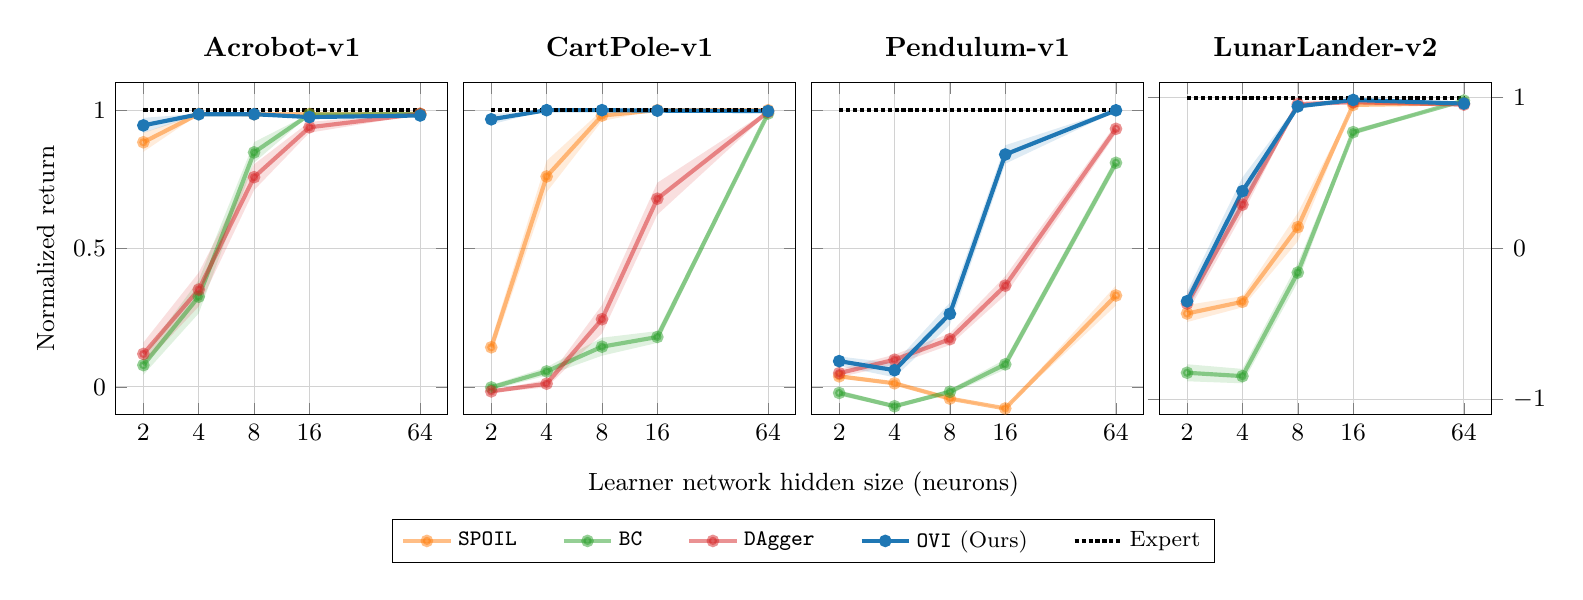
\begin{tikzpicture}
  \begin{groupplot}[
    size plot,
    group style={
      group size=4 by 1,
      horizontal sep=0.2cm,
      xlabels at=edge bottom,
      ylabels at=edge left,
    },
  ]
  \nextgroupplot[
    title={Acrobot-v1},
    ymin=-0.1,
    ymax=1.1,
    ylabel={Normalized return},
    legend to name=sharedlegend,
    legend columns=-1,
    legend style={font=\footnotesize,/tikz/every even column/.append style={column sep=0.5cm}}
  ]
    \addplot[name path=pu0, draw=none, forget plot] coordinates { (2,0.9187) (4,0.9878) (8,0.9870) (16,0.9876) (64,0.9885) };
    \addplot[name path=pl0, draw=none, forget plot] coordinates { (2,0.8494) (4,0.9851) (8,0.9836) (16,0.9840) (64,0.9854) };
    \addplot[fill=algcol0, fill opacity=0.15, draw=none, forget plot] fill between[of=pu0 and pl0];
    \addplot[algcol0, mark=*, mark size=1.5pt, line width=1.5pt, opacity=0.5] coordinates { (2,0.8841) (4,0.9864) (8,0.9853) (16,0.9858) (64,0.9869) };
    \addlegendentry{\texttt{SPOIL}}
    \addplot[name path=pu1, draw=none, forget plot] coordinates { (2,0.1139) (4,0.3864) (8,0.8845) (16,0.9863) (64,0.9875) };
    \addplot[name path=pl1, draw=none, forget plot] coordinates { (2,0.0441) (4,0.2660) (8,0.8105) (16,0.9825) (64,0.9837) };
    \addplot[fill=algcol1, fill opacity=0.15, draw=none, forget plot] fill between[of=pu1 and pl1];
    \addplot[algcol1, mark=*, mark size=1.5pt, line width=1.5pt, opacity=0.5] coordinates { (2,0.0790) (4,0.3262) (8,0.8475) (16,0.9844) (64,0.9856) };
    \addlegendentry{\texttt{BC}}
    \addplot[name path=pu2, draw=none, forget plot] coordinates { (2,0.1605) (4,0.4130) (8,0.8046) (16,0.9577) (64,0.9892) };
    \addplot[name path=pl2, draw=none, forget plot] coordinates { (2,0.0784) (4,0.2908) (8,0.7113) (16,0.9185) (64,0.9843) };
    \addplot[fill=algcol2, fill opacity=0.15, draw=none, forget plot] fill between[of=pu2 and pl2];
    \addplot[algcol2, mark=*, mark size=1.5pt, line width=1.5pt, opacity=0.5] coordinates { (2,0.1195) (4,0.3519) (8,0.7579) (16,0.9381) (64,0.9867) };
    \addlegendentry{\texttt{DAgger}}
    \addplot[name path=pu3, draw=none, forget plot] coordinates { (2,0.9723) (4,0.9869) (8,0.9886) (16,0.9783) (64,0.9835) };
    \addplot[name path=pl3, draw=none, forget plot] coordinates { (2,0.9176) (4,0.9834) (8,0.9822) (16,0.9718) (64,0.9781) };
    \addplot[fill=algcol3, fill opacity=0.15, draw=none, forget plot] fill between[of=pu3 and pl3];
    \addplot[algcol3, mark=*, mark size=1.5pt, line width=1.5pt, opacity=1.0] coordinates { (2,0.9450) (4,0.9852) (8,0.9854) (16,0.9751) (64,0.9808) };
    \addlegendentry{\texttt{OVI} (Ours)}
    \addplot[black, densely dotted, line width=1.5pt, forget plot] coordinates {(2, 1) (64, 1)};
    \addlegendimage{black, densely dotted, line width=1.5pt}
    \addlegendentry{Expert}
  \nextgroupplot[
    title={CartPole-v1},
    ymin=-0.1,
    ymax=1.1,
    yticklabels={}
  ]
    \addplot[name path=pu4, draw=none, forget plot] coordinates { (2,0.1695) (4,0.8172) (8,0.9998) (16,1.0000) (64,1.0000) };
    \addplot[name path=pl4, draw=none, forget plot] coordinates { (2,0.1172) (4,0.7038) (8,0.9611) (16,1.0000) (64,1.0000) };
    \addplot[fill=algcol0, fill opacity=0.15, draw=none, forget plot] fill between[of=pu4 and pl4];
    \addplot[algcol0, mark=*, mark size=1.5pt, line width=1.5pt, opacity=0.5] coordinates { (2,0.1434) (4,0.7605) (8,0.9805) (16,1.0000) (64,1.0000) };
    \addplot[name path=pu5, draw=none, forget plot] coordinates { (2,0.0072) (4,0.0712) (8,0.1780) (16,0.2019) (64,0.9970) };
    \addplot[name path=pl5, draw=none, forget plot] coordinates { (2,-0.0105) (4,0.0413) (8,0.1130) (16,0.1593) (64,0.9787) };
    \addplot[fill=algcol1, fill opacity=0.15, draw=none, forget plot] fill between[of=pu5 and pl5];
    \addplot[algcol1, mark=*, mark size=1.5pt, line width=1.5pt, opacity=0.5] coordinates { (2,-0.0017) (4,0.0562) (8,0.1455) (16,0.1806) (64,0.9879) };
    \addplot[name path=pu6, draw=none, forget plot] coordinates { (2,-0.0112) (4,0.0255) (8,0.2959) (16,0.7379) (64,0.9984) };
    \addplot[name path=pl6, draw=none, forget plot] coordinates { (2,-0.0207) (4,-0.0016) (8,0.1937) (16,0.6226) (64,0.9894) };
    \addplot[fill=algcol2, fill opacity=0.15, draw=none, forget plot] fill between[of=pu6 and pl6];
    \addplot[algcol2, mark=*, mark size=1.5pt, line width=1.5pt, opacity=0.5] coordinates { (2,-0.0159) (4,0.0119) (8,0.2448) (16,0.6802) (64,0.9939) };
    \addplot[name path=pu7, draw=none, forget plot] coordinates { (2,0.9857) (4,1.0000) (8,1.0000) (16,0.9999) (64,0.9999) };
    \addplot[name path=pl7, draw=none, forget plot] coordinates { (2,0.9483) (4,1.0000) (8,1.0000) (16,0.9967) (64,0.9937) };
    \addplot[fill=algcol3, fill opacity=0.15, draw=none, forget plot] fill between[of=pu7 and pl7];
    \addplot[algcol3, mark=*, mark size=1.5pt, line width=1.5pt, opacity=1.0] coordinates { (2,0.9670) (4,1.0000) (8,1.0000) (16,0.9983) (64,0.9968) };
    \addplot[black, densely dotted, line width=1.5pt, forget plot] coordinates {(2, 1) (64, 1)};
  \nextgroupplot[
    title={Pendulum-v1},
    ymin=-0.1,
    ymax=1.1,
    yticklabels={}
  ]
    \addplot[name path=pu8, draw=none, forget plot] coordinates { (2,0.0466) (4,0.0189) (8,-0.0367) (16,-0.0755) (64,0.3666) };
    \addplot[name path=pl8, draw=none, forget plot] coordinates { (2,0.0303) (4,0.0076) (8,-0.0475) (16,-0.0795) (64,0.2942) };
    \addplot[fill=algcol0, fill opacity=0.15, draw=none, forget plot] fill between[of=pu8 and pl8];
    \addplot[algcol0, mark=*, mark size=1.5pt, line width=1.5pt, opacity=0.5] coordinates { (2,0.0385) (4,0.0132) (8,-0.0421) (16,-0.0775) (64,0.3304) };
    \addplot[name path=pu9, draw=none, forget plot] coordinates { (2,-0.0116) (4,-0.0631) (8,-0.0088) (16,0.1000) (64,0.8290) };
    \addplot[name path=pl9, draw=none, forget plot] coordinates { (2,-0.0315) (4,-0.0760) (8,-0.0261) (16,0.0635) (64,0.7906) };
    \addplot[fill=algcol1, fill opacity=0.15, draw=none, forget plot] fill between[of=pu9 and pl9];
    \addplot[algcol1, mark=*, mark size=1.5pt, line width=1.5pt, opacity=0.5] coordinates { (2,-0.0216) (4,-0.0696) (8,-0.0175) (16,0.0818) (64,0.8098) };
    \addplot[name path=pu10, draw=none, forget plot] coordinates { (2,0.0644) (4,0.1169) (8,0.1938) (16,0.4003) (64,0.9499) };
    \addplot[name path=pl10, draw=none, forget plot] coordinates { (2,0.0353) (4,0.0802) (8,0.1515) (16,0.3318) (64,0.9153) };
    \addplot[fill=algcol2, fill opacity=0.15, draw=none, forget plot] fill between[of=pu10 and pl10];
    \addplot[algcol2, mark=*, mark size=1.5pt, line width=1.5pt, opacity=0.5] coordinates { (2,0.0499) (4,0.0986) (8,0.1726) (16,0.3661) (64,0.9326) };
    \addplot[name path=pu11, draw=none, forget plot] coordinates { (2,0.1102) (4,0.0863) (8,0.3045) (16,0.8732) (64,1.0033) };
    \addplot[name path=pl11, draw=none, forget plot] coordinates { (2,0.0763) (4,0.0348) (8,0.2243) (16,0.8066) (64,0.9957) };
    \addplot[fill=algcol3, fill opacity=0.15, draw=none, forget plot] fill between[of=pu11 and pl11];
    \addplot[algcol3, mark=*, mark size=1.5pt, line width=1.5pt, opacity=1.0] coordinates { (2,0.0933) (4,0.0606) (8,0.2644) (16,0.8399) (64,0.9995) };
    \addplot[black, densely dotted, line width=1.5pt, forget plot] coordinates {(2, 1) (64, 1)};
  \nextgroupplot[
    title={LunarLander-v2},
    ymin=-0.1,
    ymax=1.1,
    ymin=-1.1,
    ytick={-1,0,1},
    yticklabel pos=right,
    ytick align=outside
  ]
    \addplot[name path=pu12, draw=none, forget plot] coordinates { (2,-0.3735) (4,-0.3155) (8,0.2358) (16,0.9558) (64,0.9655) };
    \addplot[name path=pl12, draw=none, forget plot] coordinates { (2,-0.4867) (4,-0.3893) (8,0.0480) (16,0.9472) (64,0.9601) };
    \addplot[fill=algcol0, fill opacity=0.15, draw=none, forget plot] fill between[of=pu12 and pl12];
    \addplot[algcol0, mark=*, mark size=1.5pt, line width=1.5pt, opacity=0.5] coordinates { (2,-0.4301) (4,-0.3524) (8,0.1419) (16,0.9515) (64,0.9628) };
    \addplot[name path=pu13, draw=none, forget plot] coordinates { (2,-0.7661) (4,-0.7971) (8,-0.0965) (16,0.7901) (64,0.9827) };
    \addplot[name path=pl13, draw=none, forget plot] coordinates { (2,-0.8788) (4,-0.8925) (8,-0.2211) (16,0.7522) (64,0.9782) };
    \addplot[fill=algcol1, fill opacity=0.15, draw=none, forget plot] fill between[of=pu13 and pl13];
    \addplot[algcol1, mark=*, mark size=1.5pt, line width=1.5pt, opacity=0.5] coordinates { (2,-0.8225) (4,-0.8448) (8,-0.1588) (16,0.7711) (64,0.9804) };
    \addplot[name path=pu14, draw=none, forget plot] coordinates { (2,-0.3008) (4,0.3550) (8,0.9652) (16,0.9782) (64,0.9632) };
    \addplot[name path=pl14, draw=none, forget plot] coordinates { (2,-0.4283) (4,0.2266) (8,0.9483) (16,0.9608) (64,0.9435) };
    \addplot[fill=algcol2, fill opacity=0.15, draw=none, forget plot] fill between[of=pu14 and pl14];
    \addplot[algcol2, mark=*, mark size=1.5pt, line width=1.5pt, opacity=0.5] coordinates { (2,-0.3646) (4,0.2908) (8,0.9568) (16,0.9695) (64,0.9533) };
    \addplot[name path=pu15, draw=none, forget plot] coordinates { (2,-0.2842) (4,0.4719) (8,0.9559) (16,0.9891) (64,0.9688) };
    \addplot[name path=pl15, draw=none, forget plot] coordinates { (2,-0.4131) (4,0.2885) (8,0.9276) (16,0.9795) (64,0.9517) };
    \addplot[fill=algcol3, fill opacity=0.15, draw=none, forget plot] fill between[of=pu15 and pl15];
    \addplot[algcol3, mark=*, mark size=1.5pt, line width=1.5pt, opacity=1.0] coordinates { (2,-0.3486) (4,0.3802) (8,0.9417) (16,0.9843) (64,0.9602) };
    \addplot[black, densely dotted, line width=1.5pt, forget plot] coordinates {(2, 1) (64, 1)};
  \end{groupplot}
  % Centered single X-label
  \node[below=0.6cm, font=\small] at ($(group c2r1.south east)!0.5!(group c3r1.south west)$) {Learner network hidden size (neurons)};
  % Centered shared legend
  \node[below=1.2cm] at ($(group c2r1.south east)!0.5!(group c3r1.south west)$) {\pgfplotslegendfromname{sharedlegend}};
  \end{tikzpicture}
\end{document}